
\subsection{Validation d'un document XML}

%\subsubsection{Pourquoi valider ?}

%%%%% PHILIPPE: ce slide ne passe pas à la compilation
\begin{comment}
\begin{frame}[allowframebreaks]{Pourquoi chercher à valider un document XML}

\begin{center}
\begin{tikzpicture}[node distance=1.3cm,>=stealth',bend angle=45,auto]
\footnotesize
  \tikzstyle{emptyStyle}=[text width=3cm]
  \tikzstyle{doc}=[thick,draw=DarkCyan!75,fill=DarkCyan!20,minimum width=6mm, minimum height=10mm,text centered]
  \tikzstyle{appli}=[rounded corners=1mm,thick,draw=Olive!75,fill=Olive!20,text centered,text width=2cm]
  \tikzstyle{every label}=[red]

  \begin{scope}
    \node[doc](sf1) at (0,0) {  {\it Document XML}  };
   \node[appli, right= 3cm of sf1](application) {Traitement \linebreak (Application)};
    \node[emptyStyle, below= 2.8cm of sf1](comXML)  {};
    \node[emptyStyle, below= 3cm of application](comAppli)  {};
%    \node[doc,right= 0cm of appli](serial) {Serialiseur};
%    \node[emptyStyle,right= 0.8cm of serial](sf2) {\it Forme sérialisée};
    \draw[->,>=latex] (sf1) -- (application);
%    \draw[->,>=latex] (serial) -- (sf2);
\end{scope}
  \begin{pgfonlayer}{background}
    \filldraw [line width=4mm,join=round,white!20]
      (application.north  -| comAppli.west)  rectangle (comAppli.south  -| comAppli.east);
    \filldraw [line width=4mm,join=round,white!10]
      (sf1.north  -| comXML.west)  rectangle (comXML.south  -| comXML.east);
 \end{pgfonlayer}
\end{tikzpicture}
\end{center}

\pagebreak

\begin{center}
\begin{tikzpicture}[node distance=1.3cm,>=stealth',bend angle=45,auto]
\footnotesize
  \tikzstyle{emptyStyle}=[text width=3cm]
  \tikzstyle{doc}=[thick,draw=DarkCyan!75,fill=DarkCyan!20,minimum width=6mm, minimum height=10mm,text centered]
  \tikzstyle{appli}=[rounded corners=1mm,thick,draw=Olive!75,fill=Olive!20,text centered,text width=2cm]
  \tikzstyle{every label}=[red]

\begin{scope}
    \node[doc](sf1) at (0,0) {  {\it Document XML}  };
   \node[appli, right= 3cm of sf1](application) {Traitement \linebreak (Application)};
    \node[emptyStyle, below= 2.8cm of sf1](comXML)  {{\it XML $\rightarrow$ grande flexiblilité}};
    \node[emptyStyle, below= 3cm of application](comAppli)  {};
%    \node[doc,right= 0cm of appli](serial) {Serialiseur};
%    \node[emptyStyle,right= 0.8cm of serial](sf2) {\it Forme sérialisée};
    \draw[->,>=latex] (sf1) -- (application);
%    \draw[->,>=latex] (serial) -- (sf2);
\end{scope}
  \begin{pgfonlayer}{background}
    \filldraw [line width=4mm,join=round,white!20]
      (application.north  -| comAppli.west)  rectangle (comAppli.south  -| comAppli.east);
    \filldraw [line width=4mm,join=round,DarkCyan!10]
      (sf1.north  -| comXML.west)  rectangle (comXML.south  -| comXML.east);
 \end{pgfonlayer}
\end{tikzpicture}
\end{center}

\pagebreak

\begin{center}
\begin{tikzpicture}[node distance=1.3cm,>=stealth',bend angle=45,auto]
\footnotesize
  \tikzstyle{emptyStyle}=[text width=3cm]
  \tikzstyle{doc}=[thick,draw=DarkCyan!75,fill=DarkCyan!20,minimum width=6mm, minimum height=10mm,text centered]
  \tikzstyle{appli}=[rounded corners=1mm,thick,draw=Olive!75,fill=Olive!20,text centered,text width=2cm]
  \tikzstyle{every label}=[red]

  \begin{scope}
    \node[doc](sf1) at (0,0) {  {\it Document XML}  };
   \node[appli, right= 3cm of sf1](application) {Traitement \linebreak (Application)};
    \node[emptyStyle, below= 2.8cm of sf1](comXML)  {{\it XML $\rightarrow$ grande flexiblilité}};
    \node[emptyStyle, below= 3cm of application](comAppli)  {{\it Pas forcément flexible !}};
%    \node[doc,right= 0cm of appli](serial) {Serialiseur};
%    \node[emptyStyle,right= 0.8cm of serial](sf2) {\it Forme sérialisée};
    \draw[->,>=latex] (sf1) -- (application);
%    \draw[->,>=latex] (serial) -- (sf2);
\end{scope}
  \begin{pgfonlayer}{background}
    \filldraw [line width=4mm,join=round,DarkOliveGreen!20]
      (application.north  -| comAppli.west)  rectangle (comAppli.south  -| comAppli.east);
    \filldraw [line width=4mm,join=round,DarkCyan!10]
      (sf1.north  -| comXML.west)  rectangle (comXML.south  -| comXML.east);
 \end{pgfonlayer}
\end{tikzpicture}
\end{center}


\pagebreak

\begin{center}
\begin{tikzpicture}[node distance=1.3cm,>=stealth',bend angle=45,auto]
\footnotesize
  \tikzstyle{emptyStyle}=[text width=3cm]
  \tikzstyle{doc}=[thick,draw=DarkCyan!75,fill=DarkCyan!20,minimum width=6mm, minimum height=10mm,text centered]
  \tikzstyle{appli}=[rounded corners=1mm,thick,draw=Olive!75,fill=Olive!20,text centered,text width=2cm]
  \tikzstyle{every label}=[red]

  \begin{scope}
    \node[doc](sf1) at (0,0) {  {\it Document XML}  };
   \node[appli, right= 3cm of sf1](application) {Traitement \linebreak (Application)};
    \node[emptyStyle, below= 2.8cm of sf1](comXML)  {{\it XML $\rightarrow$ grande flexiblilité}};
    \node[emptyStyle, below= 3cm of application](comAppli)  {{\it Pas forcément flexible !}};
   \node[appli, left= 0cm of application, thick,draw=red,fill=red,minimum width=1mm, minimum height=10mm,text width=3mm](stop) {N \linebreak  O};
%    \node[doc,right= 0cm of appli](serial) {Serialiseur};
%    \node[emptyStyle,right= 0.8cm of serial](sf2) {\it Forme sérialisée};
    \draw[->,>=latex] (sf1) -- (stop);
%    \draw[->,>=latex] (serial) -- (sf2);
\end{scope}
  \begin{pgfonlayer}{background}
    \filldraw [line width=4mm,join=round,DarkOliveGreen!20]
      (application.north  -| comAppli.west)  rectangle (comAppli.south  -| comAppli.east);
    \filldraw [line width=4mm,join=round,DarkCyan!10]
      (sf1.north  -| comXML.west)  rectangle (comXML.south  -| comXML.east);
 \end{pgfonlayer}
\end{tikzpicture}
\end{center}


\end{frame}
\end{comment}

\begin{frame}[allowframebreaks]{La validation}

Valider :
\begin{enumerate}
\item Associer un schéma permettant d'ajouter des contraintes sur les données : 
\begin{itemize}
\item noms des éléments, 
\item sous-éléments possibles, ordre d'apparition, nombre d’occurrences,
\item attributs d'un élément,
\item type : cha\^ine, type énuméré, clef, clef étrangère,
\item occurence : obligatoire ou non,
\item valeur : par défaut ou fixée,
\item etc.
\end{itemize}
Pour XML, les schémas sont exprimés sous la forme d'une grammaire.
\item Vérifier que le document est conforme \`a la grammaire.
\end{enumerate}


\prof{faire le parallèle avec une BD}

\framebreak


\begin{block}{Objectifs}
\begin{itemize}
  \item Assurer une meilleure qualité des données transmises ou re\c{c}ues
   \item Améliorer l'interopérabilité des applications.
 \end{itemize}
\end{block}



\begin{center}
\begin{tikzpicture}[node distance=1.3cm,>=stealth',bend angle=45,auto]
\footnotesize
  \tikzstyle{emptyStyle}=[text width=3cm]
  \tikzstyle{doc}=[thick,draw=DarkCyan!75,fill=DarkCyan!20,minimum width=6mm, minimum height=10mm,text centered, ,text width=2cm]
  \tikzstyle{appli}=[rounded corners=1mm,thick,draw=Olive!75,fill=Olive!20,text centered,text width=2cm]
  \tikzstyle{every label}=[red]

  \begin{scope}
    \node[doc](sf1) at (0,0) {  {\it Document XML}   satisfaisant  un schéma $S$  };
   \node[appli, right= 3cm of sf1](application) {Traitement (Application)   sachant gérer   des documents   de schéma $S$};
  \node[appli, left= 0cm of application, thick,draw=GreenGo!75,fill=GreenGo!75,minimum width=1mm, minimum height=10mm,text width=3mm] {};
   \draw[->,>=latex] (sf1) -- (application);
\end{scope}
\end{tikzpicture}
\end{center}

\begin{block}{Document valide}
Un document est \alert{valide} s'il respecte le schéma qui lui est associé.
\end{block}

\end{frame}


\begin{frame}{Valider un document XML}

Formalismes permettant d'écrire un schéma de document(s) XML :

\begin{itemize}

\item avec une syntaxe particulière

\begin{itemize}
\item \textbf<4>{DTD (Document Type Definition)} \uncover<2->{$\leftarrow$ {\it Dans la norme XML elle-même (donc recommandé W3C)}}
\end{itemize}

\item dans un dialecte XML

\begin{itemize}
\item \textbf<4>{XML Schema} \uncover<3->{$\leftarrow$ {\it Recommandé W3C}}
\item RelaxNG, 
\item Schematron,
\item ...
\end{itemize}

\end{itemize}

Schéma exprimé sous forme d'une grammaire, décrivant la ``forme'' des arbres XML satisfaisant le schéma.

\prof{DTD : le plus ancien (première norme XML de 1998),\\
XML Schema : plus récent (2001), plus expressif\\
DTD et XML Schema sont les seuls normalisés par le W3C et les seuls qu'on étudiera\\
Nous verrons donc dans ce cours : DTD et XML Schema qui sont les deux formalismes les plus utilisés}
\end{frame}

%\subsubsection{DTD (Document Type Definition)}


\begin{frame}[containsverbatim]{Une DTD en deux mots}

Sous forme d'une grammaire :

\begin{itemize}
\item \textcolor{seaGreen}{ $\rightarrow$ simple à écrire et à comprendre},
\item \textcolor{seaGreen}{$\rightarrow$ rapide à écrire}, 
\item \textcolor{indiaRed}{$\rightarrow$ peu expressive}. \prof{une alternative sera XML Schema}
\end{itemize}

\begin{lstlisting}[caption={Exemple simple d'une DTD},numbers=left]
<!ELEMENT NEWSPAPER (ARTICLE+)>
<!ELEMENT ARTICLE (AUTHOR+,HEADLINE, BYLINE, LEAD, BODY, NOTES*)>
<!ELEMENT HEADLINE (#PCDATA)>
<!ELEMENT AUTHOR(#PCDATA)>
<!ELEMENT BYLINE (#PCDATA)>
<!ELEMENT LEAD (#PCDATA)>
<!ELEMENT BODY (#PCDATA)>
<!ELEMENT NOTES (#PCDATA)>

<!ATTLIST ARTICLE EDITOR CDATA #IMPLIED>
<!ATTLIST ARTICLE DATE CDATA #IMPLIED>
<!ATTLIST ARTICLE EDITION CDATA #IMPLIED>
\end{lstlisting}

\end{frame}



\begin{frame}[containsverbatim, allowframebreaks]{Définition d'un élément}


\begin{itemize}
\item élément vide  \verb7<!ELEMENT nom_elt EMPTY>7 

\begin{minipage}{0.9\textwidth}
\begin{exampleblock}{élément vide}
Bout de la DTD : \verb7<!ELEMENT br EMPTY>7\\
Un élément le satisfaisant : \verb7<br/>7 ou \verb?<br></br>?
\end{exampleblock}
\end{minipage}

\begin{minipage}{0.9\textwidth}
\begin{exoblock}%[Questions ...]
L'élément \verb7<BR/>7 satisfait-il le bout de DTD ci-dessus ?
\end{exoblock}
\end{minipage}

\item feuille \verb7<!ELEMENT nom (#PCDATA)>7
\begin{minipage}{0.9\textwidth}
\begin{exampleblock}{Feuille}
Bout de la DTD : \verb7<!ELEMENT auteur (#PCDATA)>7\\
Un élément le satisfaisant : \verb7<auteur>Victor Hugo</auteur>7
\end{exampleblock}
\end{minipage}

\begin{minipage}{0.9\textwidth}
\begin{exoblock}%[Questions ...]
Proposez un autre élément satisfaisant le bout de DTD ci-dessus.
\end{exoblock}
\end{minipage}

\item sans contrainte sur les sous-éléments \verb7<!ELEMENT nom ANY>7 \prof{potentiellement vide}
\begin{minipage}{0.9\textwidth}
\begin{exampleblock}{Sans contrainte sur les sous-éléments}
Bout de la DTD : \verb7<!ELEMENT auteur ANY)>7\\
Un élément le satisfaisant : \verb7<auteur>Victor Hugo</auteur>7\\
Un autre élément le satisfaisant : 
\begin{lstlisting}[language=myXML]
  <auteur>
    <prenom>Victor</prenom>
    <nom>Hugo</nom>
  </auteur>
\end{lstlisting}
\end{exampleblock}
\end{minipage}
\begin{minipage}{0.9\textwidth}

\begin{exoblock}%[Questions ...]
Proposez un autre élément satisfaisant le bout de DTD ci-dessus.
\end{exoblock}
\end{minipage}

\pagebreak

\item avec contrainte sur les sous-éléments 

\begin{small}

\begin{exampleblock}{Avec contrainte sur les sous-éléments}

Bouts de DTD : \verb7<!ELEMENT auteur (nom)>7\\
\verb7<!ELEMENT auteur (nom?)>7\\
\verb7<!ELEMENT auteur (livre*)>7\\
\verb7<!ELEMENT auteur (nom, prenom)>7\\
\verb7<!ELEMENT cours (magistral | projet)>7 \\
\verb7<!ELEMENT autheur (nom, prenom?)>7\\ 
\verb7<!ELEMENT livre (isbn,sommaire?)>7\\
\verb7<!ELEMENT livre (isbn,titre,auteur+,critiques*)>7\\
\verb7<!ELEMENT cours ((date,salle)+,(url|fichier+)+)>7
\end{exampleblock}

\medskip

Cardinalités :\\
\begin{description}
\item[(vide)] : exactement 1 occurrence 
\item[*] : 0 \`a $\infty$ occurrences 
\item[+] : 1 \`a  $\infty$ occurrences 
\item[?] : 0 ou 1 occurrence 
\end{description}

Contraintes sur la DTD : (i) 
il doit exister au plus une déclaration \verb7<!ELEMENT ..>7 par élément\,; (ii)
tous les éléments doivent \^etre définis.

\end{small}

\pagebreak

\begin{minipage}{0.9\textwidth}
\begin{exoblock}%[Questions ...]
\begin{enumerate}
\item Proposez des éléments satisfaisant chacun des bouts de DTD ci-dessus.
\item Proposez quelques définitions d'éléments avec contraintes sur les sous-éléments, et quelques éléments-instances qui pourraient satisfaire chacun d'eux.
\item Proposez deux définitions d'élément que satisfait un même élément instance.
\end{enumerate}
\end{exoblock}
\end{minipage}

\end{itemize}

\end{frame}


\begin{frame}[containsverbatim]{Simples DTD}

\begin{exoblock}%[Questions ...]
Ajoutez les cardinalités à la DTD suivante :
\begin{lstlisting}
<!ELEMENT note (to, from, heading, body)>
<!ELEMENT to (#PCDATA)>
<!ELEMENT from (#PCDATA)>
<!ELEMENT heading (#PCDATA)>
<!ELEMENT body (#PCDATA)>
\end{lstlisting}
\end{exoblock}

\end{frame}



\begin{frame}[containsverbatim]{Simples DTD}

\begin{exoblock}%[Questions ...]
Ajoutez l'information
\textit{une note contient soit un \textit{heading} soit un \textit{body}} à la DTD ci-dessous :
\begin{lstlisting}[caption={Le mémo}]
<!ELEMENT note (to+, from, heading?, body?)>
<!ELEMENT to (#PCDATA)>
<!ELEMENT from (#PCDATA)>
<!ELEMENT heading (#PCDATA)>
<!ELEMENT body (#PCDATA)>
\end{lstlisting}
\end{exoblock}

\prof{
$<!ELEMENT note (to+, from, (heading|body))>$\\
$<!ELEMENT to (\#PCDATA)>$\\
$<!ELEMENT from (\#PCDATA)>$\\
$<!ELEMENT heading (\#PCDATA)>$\\
$<!ELEMENT body (\#PCDATA)>$
}

\end{frame}


\begin{frame}[containsverbatim, allowframebreaks]{Définition d'attributs}

Rappel :
\begin{lstlisting}[caption={élément \texttt{genie} et ses attributs}]
  <genie date_naiss="1906-04-28" date_deces="1978-01-14">
      Kurt Godel
  </genie>
\end{lstlisting}

\bigskip

Pour déclarer un attribut : \\

\medskip

\begin{tabular}{ll}
\begin{minipage}{0.55\textwidth}
\begin{small}
\begin{verbatim}
<!ATTLIST nom_elt
 nom_1 type_1 occurrence_1 defaut_1  
 ...
 nom_n type_n occurrence_n defaut_n
 > 
\end{verbatim}
\end{small}
\end{minipage}
&
\begin{minipage}{0.40\textwidth}
\begin{lstlisting}
<!ATTLIST book
    ISBN CDATA #REQUIRED 
    lang (fr|en) #IMPLIED
    subject CDATA #IMPLIED>
\end{lstlisting}
\end{minipage}\\
\end{tabular}

\framebreak

\begin{tabular}{ll}
\begin{minipage}{0.55\textwidth}
\begin{small}
\begin{verbatim}
<!ATTLIST nom_elt
 nom_1 type_1 occurrence_1 defaut_1 
 ...
 nom_n type_n occurrence_n defaut_n
 > 
\end{verbatim}
\end{small}
\end{minipage}
&
\begin{minipage}{0.40\textwidth}
\begin{lstlisting}
<!ATTLIST book
    ISBN CDATA #REQUIRED 
    lang (fr|en) #IMPLIED
    subject CDATA #IMPLIED>
\end{lstlisting}
\end{minipage}\\
\end{tabular}
où\\
\begin{itemize}
\item \texttt{nom\_elt} est le nom de l'élément possédant les attributs 
\item \texttt{nom\_att\_i}  est le nom d'un attribut défini. \\
 
 \item \texttt{type\_i} est le type de l'attribut, parmi \\
  \begin{itemize}
  \item \texttt{CDATA} : cha\^ine de caractères 
  \item $(ch_1 | ... |ch_k)$ : énumération des cha\^ines de caractères  
  \item \texttt{ID} : clef
  \item \texttt{IDREF} : clef étrangère référen\c{c}ant \alert{une} clef
  \item \texttt{IDREFS} : clef étrangère référen\c{c}ant \alert{des} clefs 
   \end{itemize}

\framebreak

\item \texttt{occurence\_i}  prend sa valeur dans :
  \begin{description}
  \item[\texttt{\#REQUIRED}] = obligatoire 
  \item[\texttt{\#IMPLIED}] = optionnel 
  \item[\texttt{\#FIXED valeur}] = valeur fixée (pas de valeur par défaut)
  \item[(vide)] : par défaut, \texttt{\#REQUIRED}
  \end{description}

\item \texttt{defaut} est la valeur par défaut (si \texttt{\#FIXED}, \texttt{\#IMPLIED} ou énumération)

\end{itemize}

\prof{FIXED peut servir par exemple à imposer un espace de noms ou un auteur di fichier}

\end{frame}

\begin{frame}[containsverbatim]{Déclaration d'attributs}
Pour une DTD, 
\begin{enumerate}
\item Il ne doit exister qu'une déclaration d'élément \verb7<!ELEMENT ..>7 par élément.
\item Il peut exister plusieurs définitions \verb?ATTLIST? pour un même élément mais elles sont considérées comme une seule (fusion des définitions en une seule). \\
\prof{Rappel : il ne soit pas y avoir deux attributs de même nom (m\^eme s'ils sont déclarés dans différents \verb?ATTLIST?).}
%\item Un élément doit contenir au plus un attribut de type \verb?ID?.
\end{enumerate}
\end{frame}


\begin{frame}[containsverbatim]{DTD complète avec attribut}

\lstinputlisting[basicstyle=\tiny, language=XML,breaklines=true, firstline=4,lastline=22,numbers=left ,caption={DTD bibliothèque}]{codes/bibliotheque.xml}


\begin{exoblock}
Proposez une DTD pour notre document \texttt{movies.xml}
\end{exoblock}
\end{frame}

\begin{frame}{ID et IDREF}

Rappel (cycles précédents).\\

\begin{description}
\item[Clef] Une clef est un attribut qui distingue des ``éléments'' entre eux. \\
\prof{(d'un élément) entre parenthèses car on verra ensuite qu'en XML ce n'est pas comme en BD, c'est une clef pour tous les éléments confondus}

{\it En XML, une clef est de type \verb?ID?. La valeur de cet ID doit \^etre unique (parmis tous les ID) \textbf{dans le document}.}

\item[Clef étrangère] Une clef étrangère est un attribut prenant la valeur d’une clef. \\

{\it En XML, une clef étrangère (resp. un ensemble de clefs étrangères) est (resp. sont) déclarée(s) dans un attribut de type IDREF (resp. IDREFS).}
\end{description}
\prof{pour les néophytes, on peut le voir comme un ``pointeur'' vers une clef} 

\bigskip

{\it Attention, les notions de clef au sens XML et de clef au sens des bases de données diffèrent (questions de typage/portées de la clef) !}
\end{frame}

\begin{frame}[containsverbatim]{DTD complète avec attribut}

\begin{lstlisting}[basicstyle=\tiny, language=XML,breaklines=true,numbers=left,caption={DTD bibliothèque avec ID}]
<!DOCTYPE biblio[
          <!ELEMENT biblio (book*)>
          <!ATTLIST biblio 
                    subject CDATA #IMPLIED>
          <!ELEMENT book (author+,title,publisher,pubyear)>
          <!ATTLIST book 
                    ISBN ID #REQUIRED
                    lang (fr|en) #IMPLIED
                    subject CDATA #IMPLIED
                    abstract CDATA #IMPLIED>
          <!ELEMENT author (firstname,lastname)>
          <!ELEMENT publisher (name,place)>
          <!ELEMENT name (#PCDATA)>
          <!ELEMENT place (#PCDATA)>
          <!ELEMENT title (#PCDATA)>
          <!ELEMENT firstname (#PCDATA)>
          <!ELEMENT lastname (#PCDATA)>
          <!ELEMENT pubyear (#PCDATA)>
 ]>
\end{lstlisting}


\begin{alertblock}{Portée d'un identifiant en XML}
Spécifie un ID unique au sein du document XML entier, dont la portée est tout le document $\rightarrow$ Il ne doit pas exister
 deux valeurs identiques d'ID (\alert{tous élements confondus}) au sein d'un même document.\\
\end{alertblock}
\end{frame}

\begin{frame}[containsverbatim, fragile]{IDREF(S)}
%\begin{tabular}{ll}
\lstset{numbers=left, basicstyle=\tiny}
\begin{tabular}{p{5.5cm} l p{4cm}}
Ma DTD contient (entre autres) les déclarations d'attributs suivantes (en admettant que les éléments soient déclarés avant) :
& &
Puis-je trouver les lignes suivantes dans un fichier XML vérifiant la DTD ?
\\
%\end{tabular}
\begin{minipage}{0.5\textwidth}
\begin{lstlisting}%[basicstyle=\tiny, language=XML,breaklines=true,numbers=left]
..
<!ATTLIST square width CDATA ``0''>
..
<!ATTLIST voiture carburant (essence|diesel|hybride)> 
..
<!ATTLIST person number CDATA #REQUIRED>
..
<!ATTLIST contact fax CDATA #IMPLIED>
..
<!ATTLIST sender company CDATA #FIXED ``Microsoft''>
..
<!ATTLIST employe numsecu ID #REQUIRED>
..
<!ATTLIST livre isbn ID #REQUIRED>
..
<!ATTLIST assure person IDREF #REQUIRED>
..
\end{lstlisting}
\end{minipage}
& &
\begin{minipage}{0.35\textwidth}
\begin{lstlisting}%[basicstyle=\tiny, language=XML,breaklines=true,numbers=left]
..
<square width=''100" />
..
<person number="5677" />
..
<person />
..
<contact fax="555-667788" />
..
<contact />
..
<sender company="Microsoft" />
..
<sender company="W3Schools" />
..
<employee numsecu="1760413"/>
..
<livre isbn="978-0070507753"/>
..
<assure person="1760413">
..
<employee numsecu="978-0070507753">
..
\end{lstlisting}
\end{minipage}
\end{tabular}

\prof{l.21 non car attribut number obligatoire, l. 37 non car cette valeur d'ID existe déjà dans le fichier.}
\end{frame}

\begin{frame}[containsverbatim]{IDREF(S) (suite)}
\begin{minipage}{0.7\textwidth}

\vspace{-0.5cm}
\begin{lstlisting}[basicstyle=\footnotesize, language=XML,breaklines=true,numbers=left, label={dtdpersons1}, caption={Bout de déclaration dans une DTD}]
..
<!ELEMENT livre>
<!ATTLIST livre isbn ID #REQUIRED>
<!ELEMENT employe>
<!ATTLIST employe numsecu ID #REQUIRED>
<!ELEMENT vendeur>
<!ATTLIST vendeur person IDREF #REQUIRED>
\end{lstlisting}
\end{minipage}

\vspace{-0.7cm}

\begin{flushright}
\begin{minipage}{0.5\textwidth}
\begin{lstlisting}[basicstyle=\footnotesize, language=XML,breaklines=true,numbers=left, label={docpersons1}, caption={Bout d'instance}]
..
<employe numsecu=''1760413...''/>
<livre isbn=''978-0070507753''/>
<vendeur person=''1760413...''>
<vendeur person=''978-0070507753''>
..
\end{lstlisting}
\end{minipage}
\end{flushright}
 
\vspace{-0.5cm}
\begin{exoblock}
Le bout de document du listing \ref{dtdpersons1}  vous semble-t-il valide par rapport au bout de DTD du listing \ref{docpersons1} ? Que remarquez-vous ?
\end{exoblock}

\prof{Valide.\\
La denrière ligne est surprenante car \textit{person} pointe vers un ID de ISBN.\\
Ben oui, pas de typage, il est valide de pointer sur n'importe quel ID! Si on a dans le doc, des ID de livres, on peut pointer sur des livres sans invalider.
C'est l'une des faiblesses des DTD ça par exemple.
}
\end{frame}


\begin{frame}[containsverbatim]{IDREF(S) (suite)}
\begin{minipage}{0.7\textwidth}

\vspace{-0.5cm}
\begin{lstlisting}[basicstyle=\footnotesize, language=XML,breaklines=true,numbers=left, label={dtdpersons2}, caption={Bout de déclaration dans une DTD}]
..
<!ATTLIST livre isbn ID #REQUIRED>
..
\end{lstlisting}
\end{minipage}

\vspace{-0.7cm}

\begin{flushright}
\begin{minipage}{0.5\textwidth}
\begin{lstlisting}[basicstyle=\footnotesize, language=XML,breaklines=true,numbers=left, label={docpersons2}, caption={Bout d'instance}]
..
<livre isbn="978-0070507753"/>
   <titre>Au bonheur des dames</titre>
   <auteur>Emile Zola</auteur>
</livre>
<livre isbn="978-0070507753"/>
   <titre>L'Ecume des jours</titre>
   <auteur>Boris Vian</auteur>
</livre>
..
\end{lstlisting}
\end{minipage}
\end{flushright}
 
\vspace{-0.5cm}
\begin{exoblock}
\begin{enumerate}
\item Puis-je trouver dans un fichier XML vérifiant la DTD du listing \ref{dtdpersons2}, les éléments du listing \ref{docpersons2}?
\item Puis-je trouver ces éléments dans un fichier bien formé ? 
\end{enumerate}
\end{exoblock}

\prof{Dans un fichier bien formé oui car ne concerne pas la DTD $\rightarrow$ "on ne sait pas" que isbn est un identifiant.}
\end{frame}


\begin{frame}[containsverbatim, fragile]{Remu-méninges au cinéma...}

\begin{tabular}{cc}
\begin{minipage}{0.2\textwidth}
  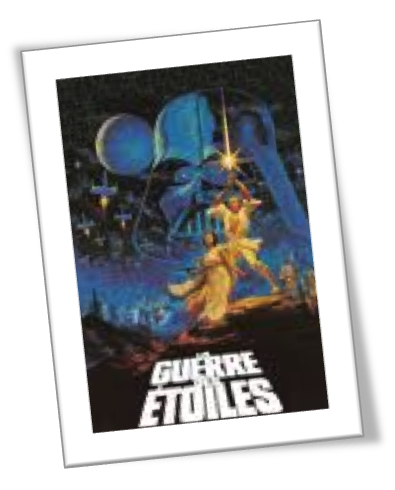
\includegraphics[width=0.95\textwidth]{images/starwars.png}\\
  
\includegraphics[width=0.9\textwidth]{images/apocalypsenow.png}
\end{minipage}
&
\begin{minipage}{0.7\textwidth}
\begin{exoblock}
\begin{enumerate}
\item Choisissez un film (f1), ainsi que deux de ses acteurs (a1 et a2).
\item Choisissez maintenant un autre film (f2) dans lequel joue a1.
\item Un film est composé d'un titre, d'une année, d'un réalisateur, et d'une liste d'acteurs. Un acteur est composé d'un nom, d'une date de naissance, et de la liste des films dans lesquels il joue. \\
\end{enumerate}

\medskip
 Proposez ensuite un fichier XML et sa DTD associée permettant de représenter ces informations avec le moins de redondance possible.
\end{exoblock}
\end{minipage}
\end{tabular}

\end{frame}

\begin{frame}[containsverbatim, fragile]{En manque d'inspiration ?}

Harrison Ford et Larry Fishburne ont tous les deux joué dans Apocalypse Now (1979, réalisation de Francis Ford Coppola).\\

Harrison Ford a également joué dans Star Wars (1977, réalisation de George Lucas).\\


\begin{tabular}{cc}
\begin{minipage}{0.45\textwidth}
 \begin{figure}
    
\includegraphics[width=0.5\textwidth]{images/fishburne.png}
    \caption{Larry Fishburne (né le 30/07/1965)}
  \end{figure}
\end{minipage}
&
\begin{minipage}{0.45\textwidth}
 \begin{figure}
    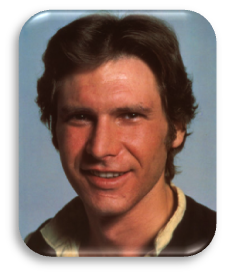
\includegraphics[width=0.5\textwidth]{images/ford.png}
    \caption{Harrison Ford (né le 13/07/1942)} \end{figure}
\end{minipage}
\end{tabular}



\prof{f1 : Apocalypse Now, 1979, réalisation de Francis Ford Coppola\\
a1 : Harrison Ford (colonel Lucas)\\
a2 : Larry Fishburne (Tyrone «Clean» Miller)\\
f2 : Star Wars, 1977, George Lucas}

\end{frame}



\begin{frame}[containsverbatim, fragile]{Remu-méninges au cinéma...}

\begin{tabular}{cc}
\begin{minipage}{0.2\textwidth}
  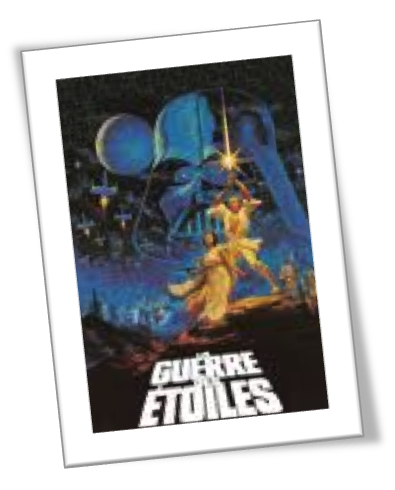
\includegraphics[width=0.95\textwidth]{images/starwars.png}\\
  
\includegraphics[width=0.9\textwidth]{images/apocalypsenow.png}
\end{minipage}
&
\begin{minipage}{0.7\textwidth}
Association plusieurs-à-plusieurs entre les entités film et acteur :
\begin{itemize}
\item à un acteur sont associés plusieurs films
\item à un film sont associés plusieurs acteurs
\end{itemize}
\end{minipage}
\end{tabular}

\medskip
\href{open : ./codes/films_le_pb.xml}{Le problème : fichier \textit{films\_le\_pb.xml}} (fichier fourni)

\href{open : ./codes/films_correction.xml}{Une correction : fichier \textit{films\_correction.xml}} (fichier fourni)
 
\end{frame}


\begin{frame}[containsverbatim, allowframebreaks]{Déclarer une DTD et l'associer à un (ou plusieurs) document(s)}

Deux fa\c{c}ons de déclarer :
\begin{itemize}
\item Déclaration interne (au fichier de données), ou
\item Déclaration externe (au fichier de données)
\end{itemize}

\framebreak

Déclaration \textbf{interne} : 
la DTD est définie dans le document lui-même.\\
\verb?<!DOCTYPE root-element [element-declarations]>?

\begin{lstlisting}[basicstyle=\footnotesize, language=XML,breaklines=true,numbers=left, caption={Déclaration interne de DTD}]
<?xml version="1.0"?>

<!DOCTYPE note [
          <!ELEMENT note (to,from,heading,body)>
          <!ELEMENT to (#PCDATA)>
          <!ELEMENT from (#PCDATA)>
          <!ELEMENT heading (#PCDATA)>
          <!ELEMENT body (#PCDATA)>
 ]>

<note>
  <to>Tove</to>
  <from>Jani</from>
  <heading>Reminder</heading>
  <body>Don't forget me this weekend</body>
</note>
\end{lstlisting}

\end{frame}

\begin{frame}[containsverbatim]{Déclarer une DTD et l'associer à un (ou plusieurs) document(s)}

Déclaration \textbf{externe} : 
la DTD est définie dans un autre document, appelé dans le document contenant les données.\\
\verb?<!DOCTYPE root-element SYSTEM "filename">?

\begin{lstlisting}[basicstyle=\footnotesize, language=XML,breaklines=true,numbers=left, caption={DTD contenue dans le fichier note.dtd}]
<!ELEMENT note (to,from,heading,body)>
<!ELEMENT to (#PCDATA)>
<!ELEMENT from (#PCDATA)>
<!ELEMENT heading (#PCDATA)>
<!ELEMENT body (#PCDATA)>
\end{lstlisting}

\begin{lstlisting}[basicstyle=\footnotesize, language=XML,breaklines=true,numbers=left, caption={Déclaration externe, fichier appelant la DTD ci-dessus}]
<?xml version="1.0"?>
<!DOCTYPE note SYSTEM "note.dtd">
<note>
  <to>Tove</to>
  <from>Jani</from>
  <heading>Reminder</heading>
  <body>Don't forget me this weekend!</body>
</note>
\end{lstlisting}

\prof{Rappel : processeur (validant ou non) met les données à disposition d'un programme (par exemple en les mettant sous forme d'arbre DOM) et le parser (validant ou non) ne fait que vérifier que le doc est bien formé (si non validant) ou valide (si valident). \\
Declaration externe souvent privilégiées pour des raisons de maintenance et de facilité d'accès. Voir avec les auditeur s'ils voient les avantages et inconvénients des deux types de déclaration.}

\end{frame}


\begin{frame}[containsverbatim, allowframebreaks]{Un exemple d'utilisation de DTD : MathML}

\begin{lstlisting}[basicstyle=\footnotesize, language=XML,breaklines=true,numbers=left]
<?xml version="1.0"?>
<math>
 <mrow>
   <msup>
     <mfenced>
       <mrow>
         <mi>a</mi>
         <mo>+</mo>      
         <mi>b</mi>
       </mrow>
     </mfenced>
     <mn>2</mn>
   </msup>
 </mrow>
</math>
\end{lstlisting}

\prof{Je dois traiter du MathML dans mon application mais je ne suis pas sur qu'il soit conforme (même si le namespace était déclaré).}

\framebreak

Vérifier qu'un document est conforme à la syntaxe MathML ?

\begin{itemize}
\item La DTD de MathML a été définie et mise en ligne à \url{http://www.w3.org/TR/MathML2/dtd/mathml2.dtd}
\item Pour s'assurer qu'un document XML est conforme à cette DTD, on peut par exemple déclarer la DTD dans de MathML celui-ci \verb?<!DOCTYPE math PUBLIC "-//W3C//DTD MathML 2.0//EN"?
         \verb?http://www.w3.org/TR/MathML2/dtd/mathml2.dtd>?
\item On teste la validité du document à l'aide d'un validateur p.e. \url{http://www.w3.org/2001/03/webdata/xsv}
\end{itemize}

\prof{Les navigateur Web ne sont pas validateurs (ils testent seulement que le doc est bien formé et ``plantent'' s'ils ne savent pas traiter le doc déclaré comme MathML mais ne respectant pas la syntaxe de MathML)}

\framebreak

\begin{lstlisting}[basicstyle=\footnotesize, language=XML,breaklines=true,numbers=left]
<?xml version="1.0"?>
<!DOCTYPE math     PUBLIC "-//W3C//DTD MathML 2.0//EN"           "http://www.w3.org/TR/MathML2/dtd/mathml2.dtd">
<math>
 <mrow>
   <msup>
     <mfenced>
       <mrow>
         <mi>a</mi>
         <mo>+</mo>      
         <mi>b</mi>
       </mrow>
     </mfenced>
     <mn>2</mn>
   </msup>
 </mrow>
</math>
\end{lstlisting}

\exo{\`A votre avis, Firefox reconnaitra-t-il maintenant du MathML ?}
\prof{Qui dit que c'est du code mathML ? On pourrait très bien utiliser ces balises pour décrire autre chose !}

\end{frame}


\begin{frame}{Vérification dynamique de schéma (typage)}
  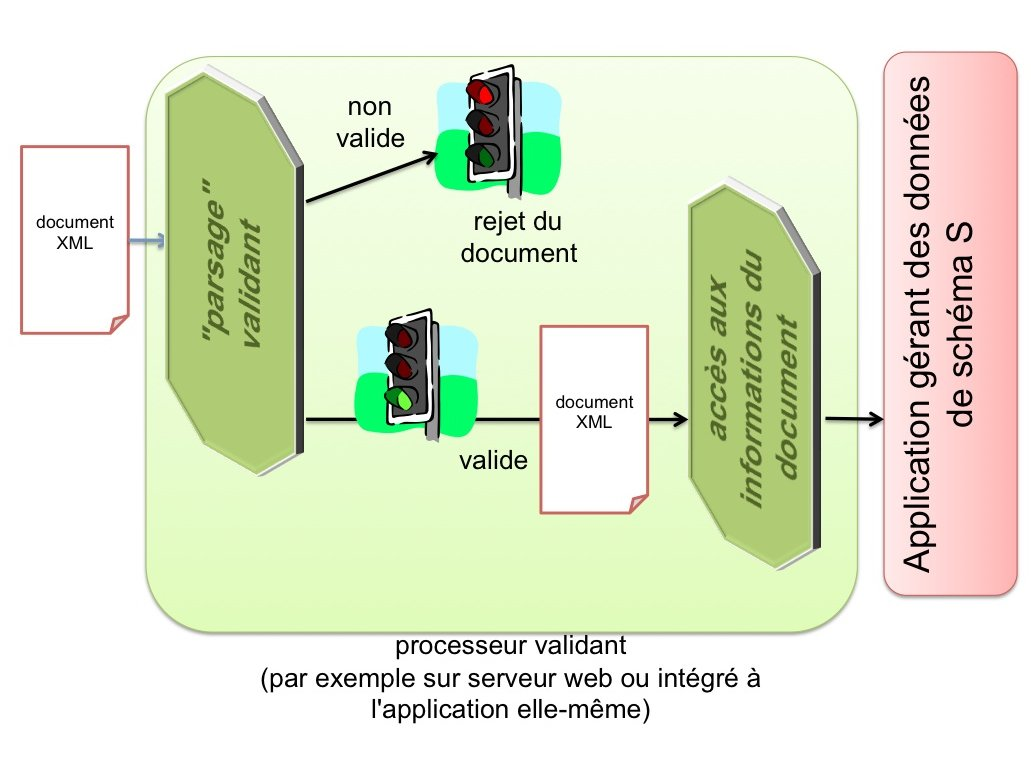
\includegraphics[width=\textwidth]{images/validation.jpg}
\end{frame}



\begin{frame}[containsverbatim]{Et la sémantique dans tout ça ?}
\begin{lstlisting}
<!DOCTYPE fiches [
	<!ELEMENT fiches (fiches*)>
          <!ELEMENT fiche (livre, auteur)>
	<!ATTLIST livre titre CDATA #REQUIRED>
	<!ELEMENT auteur (#PCDATA)>
]>
<fiches>
<fiche>
 <livre titre=''XML'' ISBN=''123456''/>
 <auteur> Martin Smith </auteur>
</fiche>
<fiche>
 <livre titre=''RDF(S)'' ISBN=''654321'' />
 <auteur> Marilyn Berton </auteur>
</fiche>
</fiches>
\end{lstlisting}

Quelle sémantique associer à ce document ?

\prof{Augmente le pouvoir d'expressivité des doc : pe ici, on sait qu'on a au moins un auteur alors que je doc sans dtd ne l'indique pas\\
Mais toujours pas de sémantique!\\
Ni avec la DTD... Ici, juste de la vérification de la structure du document. \\
Mon doc satisfait une DTD, ok, mais je ne sais toujours pas ce que les balises représentent.
}
\end{frame}



\begin{frame}{``Type ou no type ?''}

\textit{En base de données, on définit le type des données (p.e. un schéma relationnel) puis une instance de ce type (p.e. une base de données relationelles). Pour les données données semi-tructurées (et XML), les données peuvent exister avec ou sans type.}

\medskip

Les types de sont pas oubliés. Ils ne sont juste pas obligatoires. Les définir demande du temps et des efforts.  Dans certains cas, le typage n'est pas souhaité (ou pas possible) :
\begin{itemize}
\item les données sont irrégulières et la même information peut être représentée sous différentes formes (p.e. les données sont issues de différentes sources) ;
\item la structure des données est inconnue (p.e. si les données sont issues d'une source nouvellement découverte) ;
\item une partie des données est non typée (plein texte).
\end{itemize}

\begin{flushright}
Référence : \cite{WDMD}
\end{flushright}

\end{frame}


\begin{frame}{Valider ou non ?}

De plus…

\begin{itemize}
\item Valider peut être coûteux et complexe (la taille prise par la définition du schéma peut être comparable à la taille prise par les données)

\item Négociation :\\
\begin{center}
coût en temps et espace \\
vs \\
assurance de conformité au schéma (qualité)
\end{center}
\end{itemize}

\prof{discussion : si on reçoit des données extraites sont très régulièrement et pas amenées à évoluer, elles satisferont généralement le schéma. En gros, orienté document, on associe un schéma, orienté donnée, ce n'est pas toujours le cas.\\
Au delà de 100Mo la fichier, la validation peut devenir très gourmande}

\end{frame}


% \subsection{Quelques détails}


% \begin{frame}[containsverbatim]{Zoom sur les types possibles des attributs}
% \begin{description}
% \item[CDATA] type le plus permissif. On l'utilise pour des prix (chiffres suivi de devise), des URI, des emails, du texte littéraire.
% \item[NMTOKEN] cha\^ine de caractères composée uniquement de caractères alphanumériques et de points de ponctionation (\_, -, ., :). En particulier, ne contient pas d'espace. 
% \verb?<!ATTLIST livre auteur NMTOKEN>?\\
% \item[NMTOKENS] suite de NMTOKEN séparés par des espaces.
% \verb7<!ATTLIST reboot dates NMTOKENS>7\\
% \verb?<reboot dates="08-09-2010 09-09-2010 27-09-2010"/>?
% Enumeration : valeur choisie paris une liste de valeurs possibles.
% \item[ENTITY] Nom d'une entité précédemment déclarée. \prof{abbréviations genre ``SF'' pour ``Science Fiction''}
% \item[ENTITIES] Noms d'entités séparés par des espaces.
% \item[ID] clef unique (au sein du document).
% \item[IDREF] référence vers une clef du document.
% \item[IDREFS] liste de références vers des clefs du document (séparées par des espaces).
% \item[NOTATION] permet d'inclure des données non XML (p.e. images, son), en spécifiant leur format pour un futur traitement (assez peu utilisé). 
% %\verb7<!NOTATION jpeg SYSTEM "image/jpeg">7\\
% %\verb7<!NOTATION png SYSTEM "image/png">7\\
% %\verb7<!ATTLIST image type NOTATION (jpeg | png) \#REQUIRED>7
% \end{description}

% \end{frame}

% \begin{frame}[containsverbatim]{NMTOKEN}

% Un attribut peut contenir une liste de valeurs (NMTOKENS), les valeurs étant séparées par des espaces (pas d'autre séparateur possible)

% \begin{lstlisting}
% <livre>
%    <auteur>Carlo Batini</auteur>
%    <auteur>Monica Scannapieco</auteur>
%    <titre>Data quality: concepts, methodologies and techniques</titre>
%    <annee>2010<annee>
% </livre>
% \end{lstlisting}

% \begin{lstlisting}
% <livre annee=2010 auteur="Batini Scannapieco">
%    <titre>Data quality: concepts, methodologies and techniques</titre>
% </livre>
% \end{lstlisting}


% \begin{lstlisting}
% <livre annee=2010 autheur="Carlo Batini Monica Scannapieco">
%    <titre>Data quality: concepts, methodologies and techniques</titre>
% </livre>
% \end{lstlisting}
% \prof{4 tokens (4 valeurs)\\
% Nous n'irons pas jusqu'aux MNTOKENS dans le cours (\`a n'utiliser que lorsque 
% les valeurs sont séparables par un séparateur espace et qu'on veut mettre les infos dans un attribut). Contenu moins facile \`a récupérer par requ\^etage.
% }
% \end{frame}



%Elements de la biblio apparaissant pour cette section
%\nocite{WDMD,ABS99,Bri07,XML_nut,Mich99,w3c,W3Schools}

% \begin{frame}[allowframebreaks]{Références}

% \bibitem[ABS99]{ABS99}
% Serge Abiteboul, Peter Buneman, and Dan Suciu.
% \newblock {\em {Data on the Web: From Relations to Semistructured Data and
%   XML}}.
% \newblock Morgan Kaufmann, 1999.

% \bibitem[AMR04]{WDMD}
% Serge Abiteboul, Ioana Manolescu, Philippe Rigaux, Marie-Christine Rousset, and
%   Pierre Senellart.
% \newblock {\em {\textbf{Web Data Management and Distribution}}}.
% \newblock \`A paraitre, consulter le site de Philippe Rigaux
%   (\url{http://cedric.cnam.fr/~rigaux}) pour un acc\`es au matériel mis \`a
%   disposition pour le cours NFE204.

% \bibitem[Bri07]{Bri07}
% Alexandre Briant.
% \newblock {\em {XML - Cours et exercices}}.
% \newblock Eyrolles, 2007.

% \bibitem[HM04]{XML_nut}
% Elliotte~R. Harold and Scott~W. Means.
% \newblock {\em XML in a Nutshell, Third Edition}.
% \newblock {O'Reilly Media, Inc.}, 2004.

% \bibitem[Mic99]{Mich99}
% Alain Michard.
% \newblock {\em {XML, langage et applications}}.
% \newblock Eyrolles, 1999.

% \bibitem[W3C]{w3c}
% {Site du World Wide Web Consortium}.
% \newblock \url{w3c.org}.

% \bibitem[W3S]{W3Schools}
% {Site W3 Schools}.
% \newblock \url{www.w3schools.com/}.

% \bibitem[W3Cb]{w3c/dtd}
% {Site du World Wide Web Consortium, DTD}.
% \newblock \url{http://www.w3.org/TR/2008/REC-xml-20081126/#sec-prolog-dtd}.

% \bibitem[W3Cc]{w3c/ns}
% {Site du World Wide Web Consortium, namespaces}.
% \newblock \url{www.w3.org/TR/xml-names/#dt-expname}.

% \end{frame}